\documentclass[parskip=full]{scrartcl}

\pdfoutput=1

\title{Improving Imbalanced Learning in Land Cover Classification \\ 
	\LARGE{A Heuristic Oversampling Method Based on K-Means and SMOTE}}
\author{
	Georgios Douzas\(^{1}\), Fernando Bacao\(^{1*}\), Joao Fonseca\(^{1}\)
	\\
	\small{\(^{1}\)NOVA Information Management School, Universidade Nova de Lisboa}
	\\
	\small{*Corresponding Author}
	\\
	\\
	\small{Postal Address: NOVA Information Management School, Campus de Campolide, 1070-312 Lisboa, Portugal}
	\\
	\small{Telephone: +351 21 382 8610}
}

\usepackage{breakcites}
\usepackage{float}
\usepackage{graphicx}
\usepackage{geometry}
\geometry{
	a4paper,
	left=18mm,
	right=18mm,
	top=8mm,
}
\usepackage{amsmath}
\newcommand{\inlineeqnum}{\refstepcounter{equation}~~\mbox{(\theequation)}}
\usepackage{enumitem}
\usepackage[ruled,vlined]{algorithm2e}
\usepackage{booktabs}
\usepackage{pgfplotstable}
\pgfplotsset{compat=1.14}
\usepackage{longtable}
\usepackage{tabu}
\usepackage{hyperref}
\date{}

\begin{document}

\maketitle

\begin{abstract}
	TODO TODO TODO TODO TODO TODO TODO TODO TODO TODO TODO TODO TODO TODO TODO TODO
	TODO TODO TODO TODO TODO TODO TODO TODO TODO TODO TODO TODO TODO TODO TODO TODO
	TODO TODO TODO TODO TODO TODO TODO TODO TODO TODO TODO TODO TODO TODO TODO TODO
	TODO TODO TODO TODO TODO TODO TODO TODO TODO TODO TODO TODO TODO TODO TODO TODO
	TODO TODO TODO TODO TODO TODO TODO TODO TODO TODO TODO TODO TODO TODO TODO TODO
	TODO TODO TODO TODO TODO TODO TODO TODO TODO TODO TODO TODO TODO TODO TODO TODO
	TODO TODO TODO TODO TODO TODO TODO TODO TODO TODO TODO TODO TODO TODO TODO TODO
\end{abstract}

\section{Introduction}

% context

The increasing amount of remote sensing missions granted the access to dense
time series (TS) data at a global level and provides up-to-date, accurate land
cover information \cite{Drusch2012}. This information is often
materialized through Land Use/Land Cover (LULC) maps, which constitute an
essential asset for various purposes, such as land cover change detection,
urban planning, environmental monitoring and natural hazard assessment
\cite{Khatami2016}. However, the production of accurate, updated LULC maps
still pose a challenge within the remote sensing community
\cite{Wulder2018}. They can have either one of two sources:
Photo-interpreted by the human eye, or Automatic mapping using remotely sensed
data and a classification algorithm.

Although photo-interpreted LULC maps rely on human interaction and can be more
reliable, they are not without its drawbacks: they are not frequently updated,
their production is time and resource consuming, not suitable for operational
mapping over large areas and are prone to overlook rare or small-area classes,
due to factors such as the minimum mapping unit being used. Concurrently,
machine-learning (ML) approaches face different challenges:
\begin{enumerate}
	\item Mislabelled LULC patches. As mentioned, the usage of photo-interpreted training
	      data poses a threat to the quality of any LULC map produced with this strategy,
	      since factors such as the minimum mapping unit tend to cause the overlooking of
	      small-area LULC patches and generates noisy training data that may reduce the
	      prediction power of a classifier \cite{Pelletier2017}.
	\item High-dimensional datasets. Multi-spectral TS composites are high-dimensional,
	      which increases the complexity of the problem and creates a strain on
	      computational power \cite{Stromann2020}.
	\item Class separability. The production of an accurate LULC map can be hindered by
	      the existence of classes with similar spectral signatures, making these classes
	      difficult to distinguish \cite{Alonso-Sarria2019}.
	\item Existence of rare land cover classes. Due to the varying levels of area
	      coverage for each class, using a purely random sampling strategy will amount to
	      a dataset with a roughly proportional class distribution as the one on the
	      landscape. On the other hand, the acquisition of training datasets containing
	      balanced class frequencies is often unfeasible. This causes an asymmetry in
	      class distribution, where some classes are frequent in the training dataset,
	      while others have little expression \cite{Wang2019, Feng2019}.
\end{enumerate}

% problem definition

The latter challenge is known, in the machine learning community, as the
imbalanced learning problem \cite{Chawla2004}. It is defined as a skewed
distribution of observations found in a dataset among classes in both binary
and multi-class problems \cite{Abdi2016}. This asymmetry in class
distribution negatively impacts the performance of classifiers, especially in
multi-class problems. During the learning phase, classifiers are optimized to
best fit an objective function, being the most common overall accuracy
\cite{Maxwell2018}. This means that observations belonging to rare/minority
classes contribute less towards the predictive power of the corresponding
classes and will induce a bias towards majority classes, as depicted in figure
\ref{fig:oversampling_decision_function}a. As an example, a trivial classifier can achieve 99\%
overall accuracy on a binary dataset where 1\% of the observations belong to
the minority class if it classifies all observations as belonging to the
majority class.

Typical ML algorithms are designed to perform well on relatively balanced
datasets. Although, defining a decision boundary on imbalanced datasets is a
difficult task since each class' weight in the learning phase is typically as
high as its relative number of observations within the training dataset.

There are three different types of approaches to deal with the class imbalance
problem \cite{Fernandez2013,Kaur2019}:
\begin{enumerate}
	\item Cost-sensitive solutions. Introduces a cost matrix to the learning phase with
	      misclassification costs attributed to each class. Minority classes will have a
	      higher cost than majority classes, forcing the algorithm to be more flexible
	      and adapt better to predict minority classes.
	\item Algorithmic level solutions. Specific classifiers are modified to reinforce the
	      learning on minority classes. Consists on the creation or adaptation of
	      classifiers.
	\item Resampling solutions. Rebalances the dataset's class distribution by removing
	      majority class instances and/or generating artificial minority instances (see
	      Figure \ref{fig:oversampling_decision_function}). This is considered an external  approach, where
	      the intervention occurs before the learning phase, benefitting from versatility
	      and independency from the classifier used.
\end{enumerate}

Within resampling approaches there are three subgroups of approaches
\cite{Fernandez2013,Kaur2019,Luengo2020}:
\begin{enumerate}
	\item Undersampling methods. They rebalance class distribution by removing instances
	      from the majority classes.
	\item Oversampling methods. Dataset is rebalanced by generating new artificial
	      instances belonging to the minority classes.
	\item Hybrid methods. Combination of both oversampling and undersampling, resulting
	      in the removal of instances in the majority classes and the generation of
	      artificial instances in the minority classes.
\end{enumerate}

Resampling methods can be further distinguished between non-informed and
heuristic (i.e., informed) resampling techniques \cite{Fernandez2013,Luengo2020,Garcia2016}. The
former consist of methods that duplicate/remove a random selection of data
points to set class distributions to user-specified levels, and are therefore a
simpler approach to the problem. The latter consists of more sophisticated
approaches that aim to perform over/undersampling based on the points'
contextual information within their data space.

\begin{figure}[H]
	\centering
	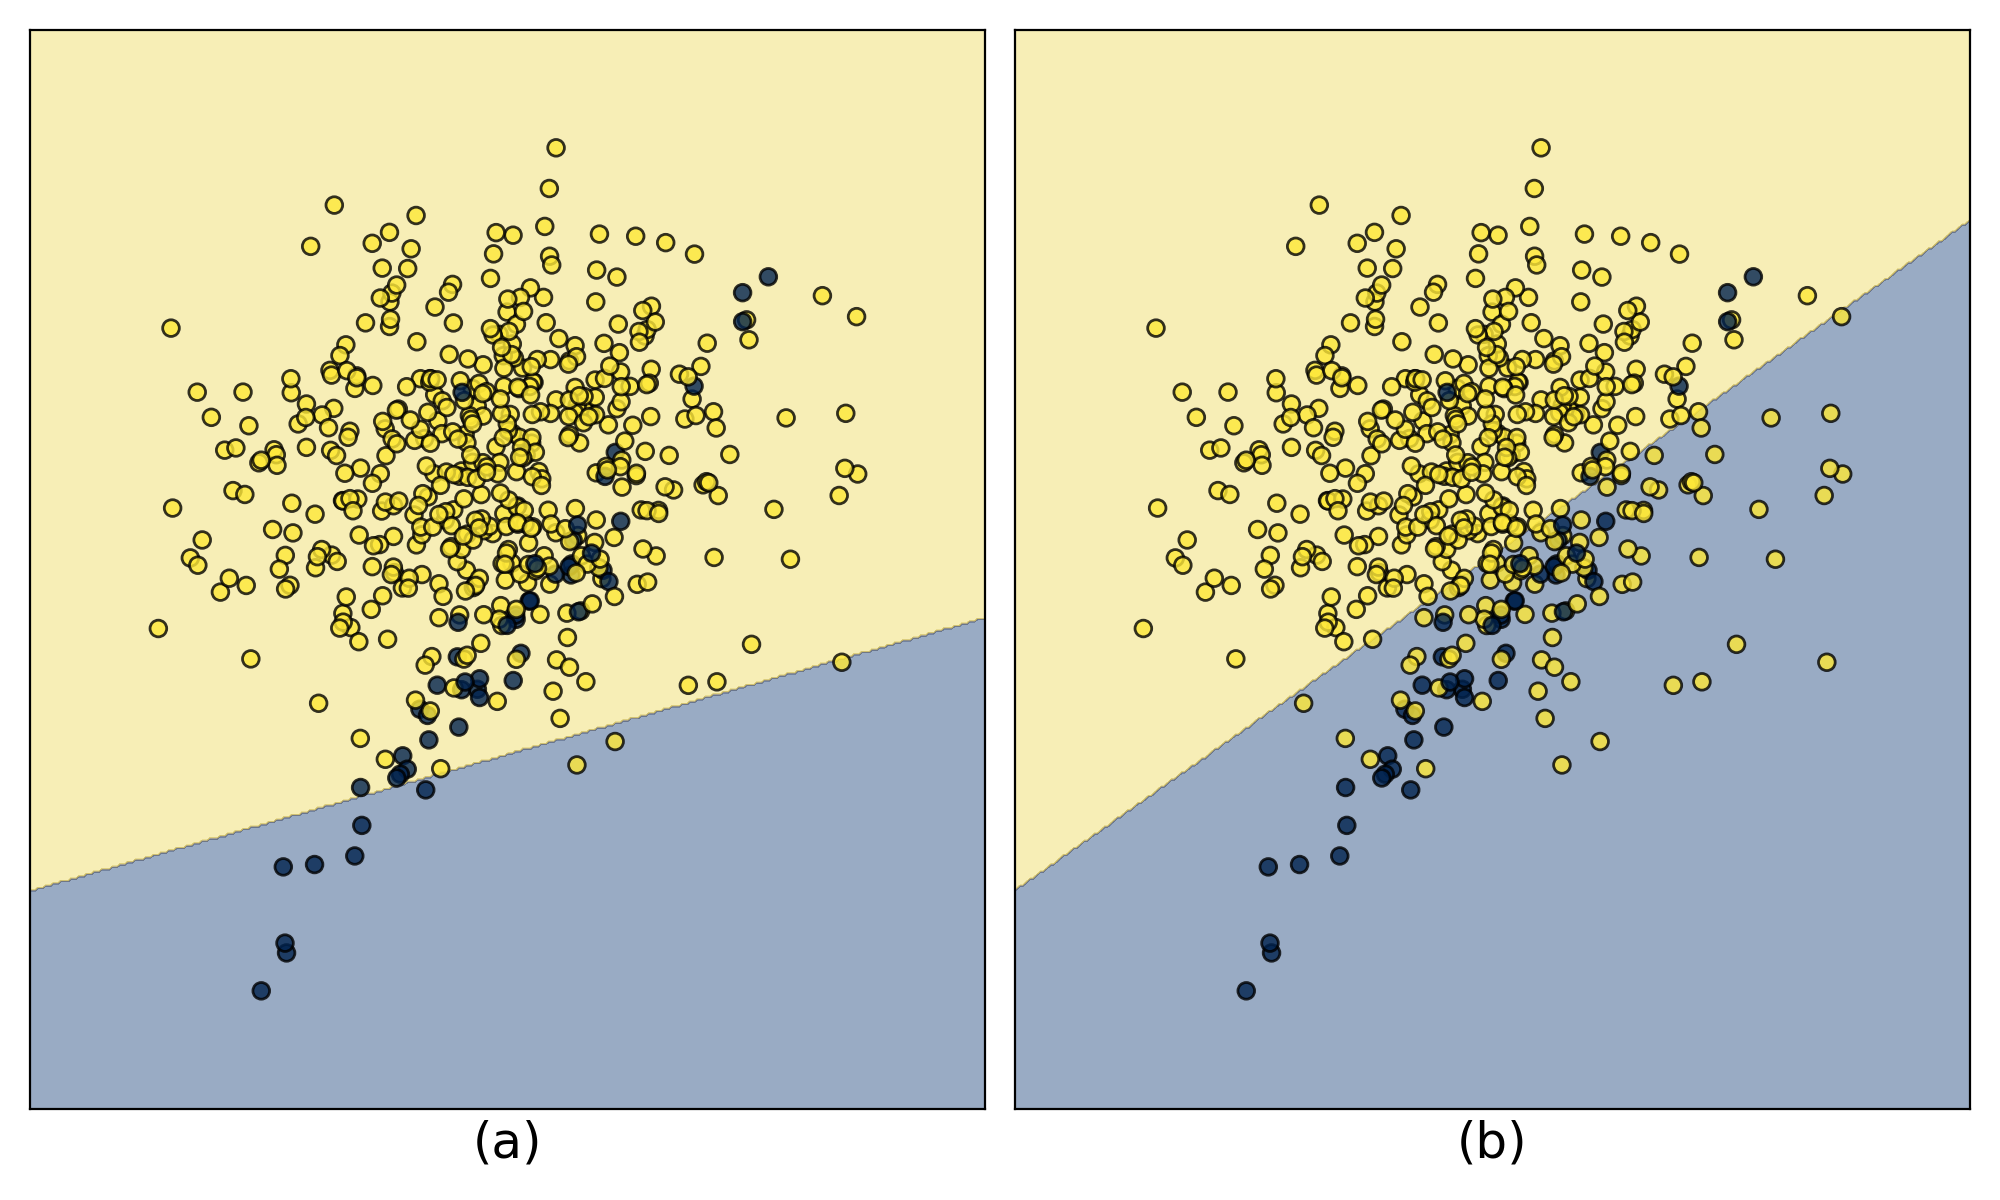
\includegraphics[width=.75\linewidth]{../analysis/oversampling_decision_function}
	\caption{Example of a linear Support Vector Machine's decision function (a) before
		resampling and (b) after resampling.}
	\label{fig:oversampling_decision_function}
\end{figure}

In this paper, we propose the K-means SMOTE (K-SMOTE) \cite{Douzas2018}
oversampler to address the imbalanced learning problem in a multiclass context
for LULC classification in various reference remote sensing datasets, as well
as a dataset extracted from publicly available portuguese LULC maps provided by
Direção Geral do Território with Sentinel-2 data. K-SMOTE's efficacy is tested
using different types of classifiers. To do so, we employ both commonly used
and state-of-the-art oversamplers as benchmarking methods: Random oversampling
(ROS), Synthetic Minority Oversampling Technique (SMOTE)
\cite{Chawla2002}, Adaptive Synthetic Sampling (ADASYN)
\cite{HaiboHe2008}, Borderline-SMOTE (B-SMOTE) \cite{Han2005} and
Geometric-SMOTE (G-SMOTE) \cite{Douzas2019}. As a baseline we present
classification results without the employment of any resampling method.

% TODO: decide on the datasets

This paper is organized in \# sections: (TODO)

\section{Imbalanced Learning Approaches}

Existing methods that address imbalanced learning act on different stages. They
can act in the preprocessing step (Over/Undersampling and hybrid approaches),
in the learning process (cost-sensitive solutions) or in the algorithm itself
(by adapting existing algorithms and/or ensemble methods)
\cite{Kaur2019}. In this section, we focus on previous work related with
resampling methods, while providing a brief explanation of cost-sensitive and
algorithmic level solutions.

All of the most common classifiers used for LULC classification tasks
\cite{Khatami2016, Gavade2019} are sensitive to class imbalance \cite{Blagus2010}.
Algorithm-based approaches typically focus on adaptations based on ensemble
classification methods \cite{Mellor2015} or common non-ensemble based
classifiers such as Support Vector Machines \cite{Shao2014}. In
\cite{Lee2016}, the reported results show that algorithm-based methods
have comparable performance to resampling methods.

Cost-sensitive solutions refer to changes in the importance attributed to each
instance through a cost matrix \cite{Huang2016,Cui2019,Dong2017}. A common cost sensitive
solution is found in \cite{Huang2016}. The authors use the inverse class
frequency (i.e., $1/|C_i|$) to give higher weight to minority
classes. Cui et al. \cite{Cui2019} extended this method by adding a
hyperparameter $\beta$ to class weights as
$(1-\beta)/(1-\beta^{|C_i|})$. When $\beta=0$, the weights are equal for
all classes. When $\beta=1$, the weights are differentiated as in
the original paper. Another method \cite{Dong2017} explores adaptations
of Cross-entropy classification loss by adding different formulations of class
rectification loss.

Imbalanced Learning is most commonly addressed through data resampling in
machine learning in general and remote sensing in particular
\cite{Feng2019}. The generation of artificial instances (i.e.,
augmenting the dataset) based on rare examples is done independently of any
other classification and preprocessing step. Once this step is applied, any
standard ML procedure can be applied. This simplicity makes resampling
strategies particularly appealing for any user interested in applying several
classifiers or maintaining a simple approach. Additionally, any of these
methods can be naturally applied to multiclass problems and particularly to
LULC classification tasks.

\subsection{Non-informed resampling methods}

There are two main non-informed resampling methods. Random Oversampling (ROS)
generates artificial observations through random duplication of rare instances.
This method is used in remote sensing \cite{Sharififar2019, Hounkpatin2018} for its
simplicity, even though its mechanism makes the classifier prone to overfitting
\cite{Krawczyk2016}. Hounkpatin et al. \cite{Hounkpatin2018} found that
using ROS returned worse results than keeping the original imbalance in their
dataset.

A few of the recent remote sensing studies employed Random Undersampling (RUS)
\cite{Ferreira2019}. This method, on the other hand, randomly removes
observations belonging to common classes. Although it's not as prone to
overfitting as ROS, it incurs into information loss by eliminating observations
from the majority class \cite{Feng2019}.

Another downfall of non-informed resampling methods is their performance-wise
inconsistency across classifiers. ROS' impact on the Indian Pines dataset was
found inconsistent between Random Forest Classifiers (RFC) and Support Vector
Machines (SVM) and lowered the predictive power of an artificial neural network
(ANN) \cite{Maxwell2018}. Similarly, RUS is found to generally lead to a
lower overall accuracy due to the associated information loss
\cite{Maxwell2018}.

\subsection{Heuristic methods}

The methods presented in this section appear as a means to overcome the
insufficiencies found in non-informed resampling. They use either local or
global information to generate new, relevant, non-duplicated instances to
populate the minority classes and/or remove irrelevant instances from majority
classes. In a comparative analysis between over- and undersamplers' performance
for LULC classification \cite{Feng2018} using the rotation forest
ensemble classifier, authors found that oversampling methods consistently
outperform undersampling methods. Due to the scope of this study, heuristic
undersampling algorithms will not be analysed.

% Are we using only oversamplers or both? This is important to know whether 
% to focus the Related Work on Oversampling only or both

SMOTE \cite{Chawla2002} was the first heuristic oversampling algorithm to
be proposed and has been the most popular one since then, likely due to its
fair degree of simplicity and quality of generated data. It takes a random
minority class sample and introduces synthetic examples along the line segments
that join any/all of the $k$ minority class nearest
neighbors to the selected sample. Specifically, a single synthetic sample
$\overrightarrow{z}$ is generated within the line segment of a randomly
selected minority class observation $\overrightarrow{x}$ and one of its
$k$ nearest neighbors $\overrightarrow{y}$ such that
$\overrightarrow{z} =
	\alpha\overrightarrow{x}+(1-\alpha)\overrightarrow{y}$, where $\alpha$ is a random floating point
between 0 and 1, as shown in Figure \ref{fig:smote_example}.

\begin{figure}[H]
	\centering
	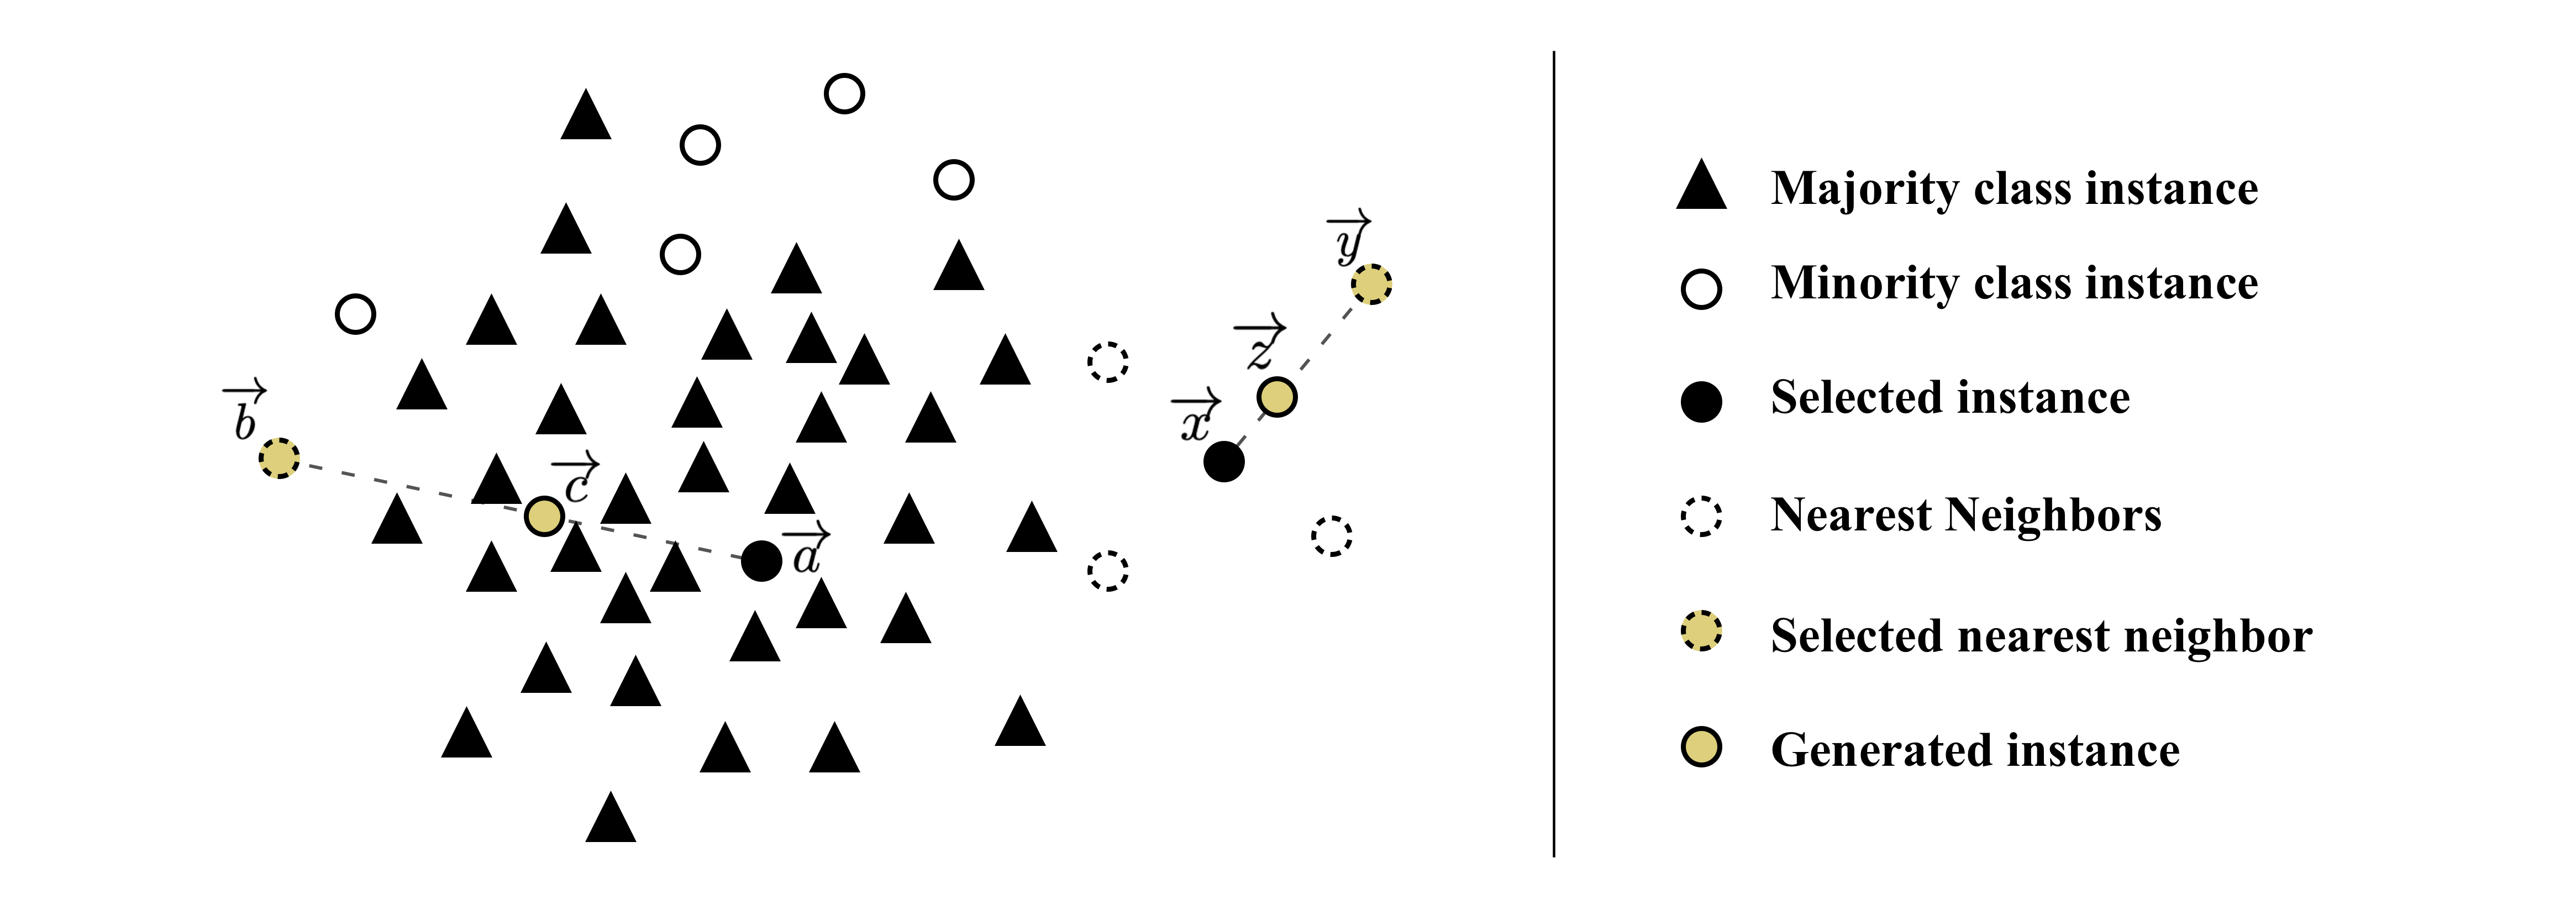
\includegraphics[width=1\linewidth]{../analysis/smote_example}
	\caption{Example of SMOTE's data generation process.}
	\label{fig:smote_example}
\end{figure}

A number of studies implement SMOTE within the LULC classification context and
reported improvements on the quality of the trained predictors
\cite{Jozdani2019, Bogner2018}. Another study proposes an adaptation of SMOTE on an
algorithmic level for deep learning applications \cite{Zhu2020}. This
method combines both typical computer vision data augmentation techniques, such
as image rotation, scaling and flipping on the generated instances to populate
minority classes. Another algorithmic implementation is the variational
semi-supervised learning model \cite{Cenggoro2018}. It consists of a
generative model that allows learning from both labelled and unlabelled
instances while using SMOTE to balance the data.

Despite SMOTE's popularity, its drawbacks motivated the development of more
sophisticated oversampling algorithms \cite{Douzas2019}:
\begin{enumerate}
	\item Generation of noisy instances due to random selection of a minority observation
	      to oversample. The random selection of a minority observation makes SMOTE
	      oversampling prone to the amplification of existing noisy data. In Figure
	      \ref{fig:smote_example} it is possible to observe a minority sample located
	      within a cluster of majority instances. Performing a linear interpolation
	      between the noisy sample $\overrightarrow{a}$ and one of its nearest neighbors
	      $\overrightarrow{b}$ will generate a noisy sample $\overrightarrow{c}$.
	      B-SMOTE \cite{Han2005} attempts to circumvent the noisy data selection
	      problem by performing a targeted selection of instances close to the presumed
	      class border, determined by the labels of each sample's $k$
	      nearest neighbors. Alternatively, a sample will discarded because it was deemed
	      as either noisy, or being far from the class boundary. Another algorithm that
	      addresses this problem is ADASYN \cite{HaiboHe2008}. It calculates a
	      density distribution ratio for each sample based on its
	      $k$-nearest neighbors to determine the number of synthetic
	      observations to generate for each minority class observation using the
	      described SMOTE procedure.

	\item Generation of noisy instances due to the selection of the $k$
	      nearest neighbors. In the event an observation (or a small number thereof) is
	      not noisy but is isolated from the remaining clusters, known as the "small
	      disjuncts problem" \cite{holte1989}, much like sample
	      $\overrightarrow{b}$ from Figure \ref{fig:smote_example}, the selection of any
	      nearest neighbor of the same class will have a high likelihood of producing a
	      noisy sample.

	\item Generation of nearly duplicated instances. Whenever the linear interpolation is
	      done between two observations that are close to each other, the generated
	      instance becomes very similar to its parents and increases the risk of
	      overfitting. G-SMOTE \cite{Douzas2019} attempts to address both the
	      $k$ nearest neighbor selection mechanism problem as well as
	      the generation of nearly duplicated instances problem. It proposes a variation
	      on SMOTE's data generation mechanism by generating data within an oval geometry
	      (instead of a line segment) around the selected observation and the selected
	      nearest neighbor. In its turn, the $k$ nearest neighbors
	      selection can include observations from the remaining classes. To an extent,
	      this algorithm can be considered a generalized version of SMOTE, since under
	      specific hyperparameter definitions it replicates SMOTE's behavior.

	\item Generation of noisy instances due to the use of observations from two different
	      minority class clusters. Although an increased $k$ could
	      potentially avoid the previous problem, it can also lead to the generation of
	      artificial data between different minority clusters. Cluster-based oversampling
	      methods, as well as ADASYN, attempt to address this problem. B-SMOTE
	      \cite{Han2005} and G-SMOTE also address this problem by allowing the
	      interpolation to be performed with majority class instances.
\end{enumerate}

Although no cluster-based oversampling approach applied within the remote
sensing domain was found in the literature, there are numerous methods to
consider. Cluster-based oversampling approaches introduce an additional layer
to SMOTE's selection mechanism, which is done according to the clustering
process. This is done to ensure both between-class data balance, but also
ensure that the data distribution within each class is preserved. The
self-organizing map oversampling (SOMO) \cite{Douzas2017} algorithm
transforms the dataset into a 2-dimensional input, where the areas with the
highest density of minority samples are identified. SMOTE is then used to
oversample each of the identified areas separately. CURE-SMOTE
\cite{Ma2017} applies a hierarchical clustering algorithm (CURE) to
discard isolated minority instances before applying SMOTE. Although it avoids
noise generation problems, it ignores within-class data distribution. Another
method \cite{Santos2015} uses K-means to cluster the entire input space
and applies SMOTE to clusters the the fewest representations, regardless of the
observations' class label. The label of the generated observation is copied
from one of its parents. This method cannot ensure a balanced dataset, class
imbalance is not specifically addressed, but rather dataset imbalance.

K-SMOTE \cite{Douzas2018} avoids noisy data generation by employing
$k$-means clustering to identify safe areas using
cluster-specific Imbalance Ratio (defined by $\frac{count(C_{majority})}{count(C_{minority})}$) and
determine the quantity of generated samples per cluster based on a density
measure. These samples are finally generated using the SMOTE algorithm. The
K-SMOTE's data generation process is depicted in Figure \ref{fig:kmeans_smote_example}.
Note that the number of samples generated for each cluster varies according to
the sparsity of each cluster (the sparser the cluster is, the more samples will
be generated) and a cluster is rejected if the cluster's IR surpasses the
threshold.

\begin{figure}[H]
	\centering
	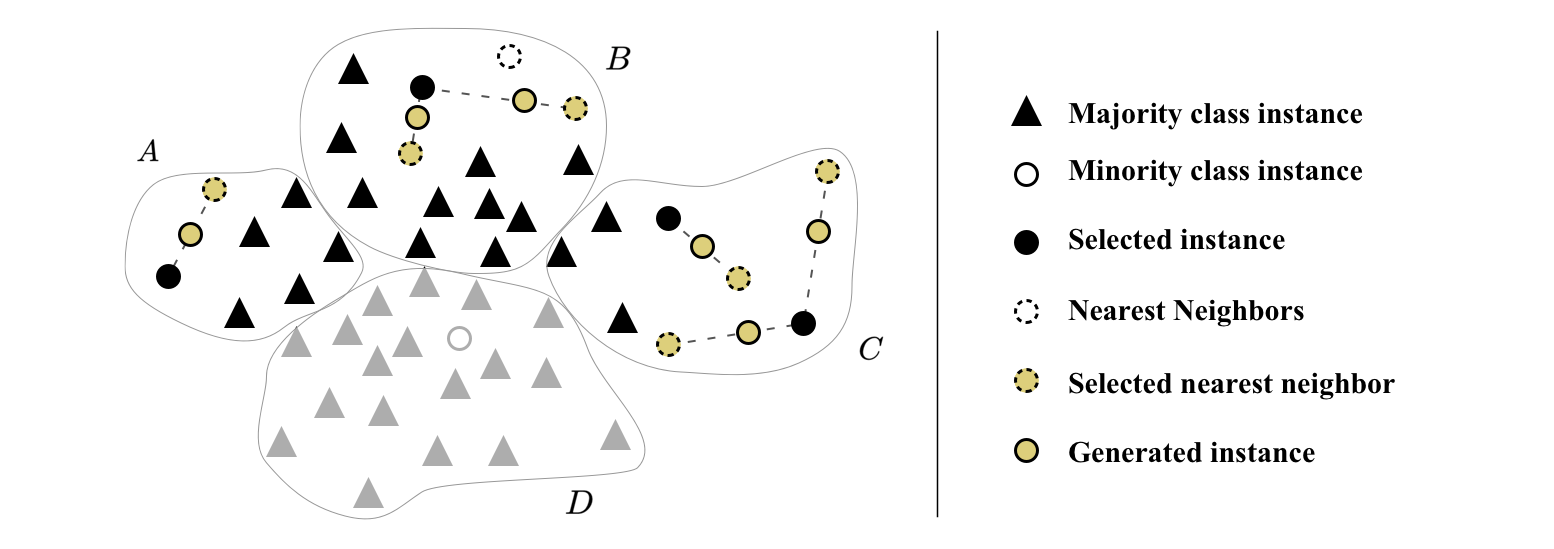
\includegraphics[width=1\linewidth]{../analysis/kmeans_smote_example}
	\caption{Example of K-SMOTE's data generation process. Clusters $A$,
		$B$ and $C$ are selected for
		oversampling, whereas cluster $D$ was rejected due to its
		high imbalance ratio. The oversampling is done using the SMOTE algorithm and
		the $k$ nearest neighbors selection only considers
		observations within the same cluster.}
	\label{fig:kmeans_smote_example}
\end{figure}

Although no other study was found to implement cluster-based oversampling,
another study \cite{Douzas2019rs} compared the performance of SMOTE, ROS,
ADASYN, B-SMOTE and G-SMOTE in a highly imbalanced LULC classification dataset.
The authors found that G-SMOTE consistently outperformed the remaining
oversampling algorithms regardless of the classifier used.

This paper main contributions are:
\begin{itemize}
	\item Testing these oversampling methods in multiple widely used LULC classification
	      datasets, as well as an additional real case dataset. Allows us to check for
	      oversamplers' performance statistical significance across datasets and report
	      K-SMOTE's performance in a real case dataset.
	\item Introducing a cluster-based oversampling algorithm within the remote sensing
	      domain, as well as comparing its performance with the remaining oversamplers in
	      a multiclass context.

\end{itemize}

\section{Methodology}

In this section we describe our experiment's settings. We provide a description
of the datasets, evaluation metrics, oversamplers, classifiers, software used
and procedure developed.

\subsection{Datasets}

\bibliography{references}
\bibliographystyle{apalike}

\end{document}
